\subsection{Label-budget repetitions}\label{app:labelbudget}
The label-efficiency experiment of Section~\ref{sec:pairresults}
retrains response supervision at the selected weight with per-query
derivative-center budgets of $6$, $12$, $24$ and $48$ centers (36--288
in total against the full 384). Each budget uses three independent
query-balanced random nested subsets: for replication $\rho$ and query
$j$, a fresh permutation of that query's $64$ training centers is drawn
from $\mathrm{rng}(20261101+\rho+97j)$, and the budget-$b$ subset is
the first $b$ entries, so the subsets of different budgets nest within
a replication while different replications are independent. Training
follows the continuation protocol of Appendix~\ref{app:pairs-v102}
unchanged (shared flow data and minibatch sequence, 1{,}200 updates,
uniform selection rule); only the derivative-label pool shrinks. The
reported curves aggregate hierarchically: within each subset
replication, the median over the 96 test paths; across the three
replications, the median of those three medians, with the shaded band
spanning their interquartile range. The full-budget point (384
centers) is the single run with the complete label set and carries no
subset variation. Across all budgets the interquartile range
stays within $0.8$ percentage points for the column error and within
$0.4$ for the family-boundary error, and flow accuracy stays within
$0.027$--$0.031\%$.

\begin{figure}[t]
\centering
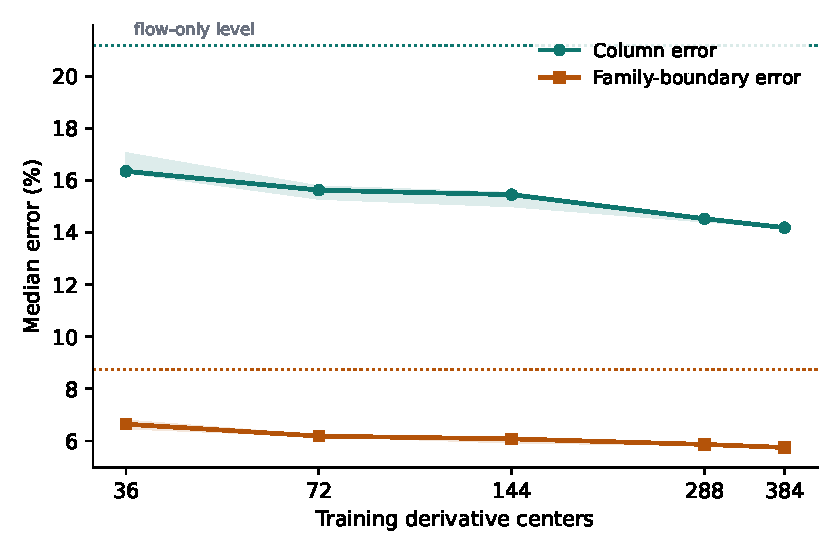
\includegraphics[width=0.72\linewidth]{../figures/fig_v111_labelbudget.pdf}
\caption{Response supervision under reduced label budgets on the 96
test paths, at the validation-selected weight: median attribution
column and family-boundary errors against the number of training
derivative centers (36--384; logarithmic axis), aggregated as stated
above (shaded: interquartile range over the three subset replications;
the 384-center point is the single full-label run), with the flow-only
levels marked (dotted).}\label{fig:v109labelbudget}
\end{figure}
